\documentclass[12pt,a4paper]{article}
\usepackage{ccicons}
\usepackage{hyperref}
\usepackage{minted}
\usepackage{graphicx}
\usepackage{booktabs}

\usepackage{./tikzit}

\setminted{autogobble=true, tabsize=2, linenos=true, frame=single, breaklines=true}

\newcommand{\version}{v0.11}


\begin{document}
\begin{centering}

	\Large{Workshop Paper}
	\par
	\Huge{Debugging of RxJS-based Applications}
	\par
	\vspace{2ex}

	\normalsize{
		Manuel Alabor\\
		Supervised by Prof. Dr. Markus Stolze\\
		\par
		\vspace{2ex}
		HSR University of Applied Sciences Rapperswil, Switzerland\\
		\par
		\vspace{2ex}
		\today{} (\version)
	}
	\par
	\vspace{2ex}

	\begin{quotation}
		\small{
			\noindent\textbf{Abstract}---RxJS is a popular library to implement data-flow-oriented applications with JavaScript using reactive programming principles. This way of programming bears new challenges for traditional debuggers: Their focus on imperative programming limits their applicability to problems originated in the declarative programming paradigm. The goals of this paper are: (i) to understand how software engineers debug RxJS-based applications, what tools do they use, what techniques they apply; (ii) to understand what are the most prevalent challenges they face while doing so; and (iii) to provide a course of action to resolve these challenges in a future iteration on the topic. We learned about the debugging habits of ten professionals using interviews, and hands-on war story reports. Based on this data, we designed and executed an observational study with four subjects to verify that engineers predominantly augment source code with manuel trace logs instead of using specialized debugging utilities. In the end, we identified the lack of fully integrated RxJS-specific debugging solutions in existing development environments as the most significant reason why engineers do not make use of such tools. We decided to elaborate on how to resolve this situation in our future work.
		}
		\par
		\vspace{4ex}
	\end{quotation}
\end{centering}

\section{Introduction}

The (graphical) user interface (\emph{UI} or \emph{GUI}) of an application handles two constant flows of data: External user input (e.g. mouse, touch or keyboard interaction) is interpreted and forwarded to the system. Once the system processed an interaction and updated its internal state accordingly, it notifies the UI about these changes which are relayed to the user.

\begin{figure}[H]
	\centering
	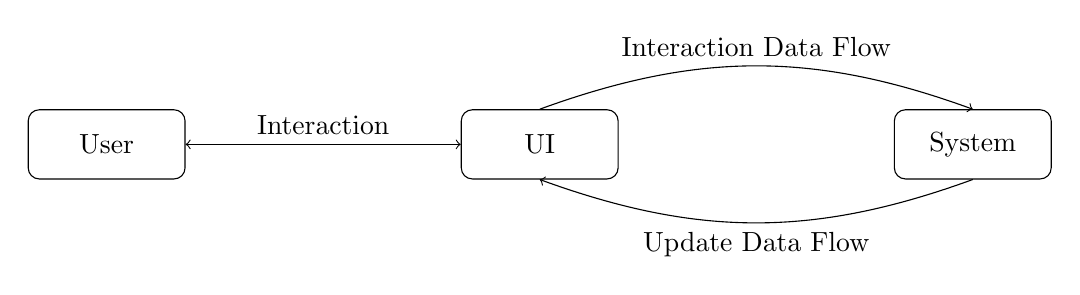
\begin{tikzpicture}[node distance = 5.5cm, auto]
		\tikzstyle{block} = [rectangle, draw,
		text width=5em, text centered, rounded corners, minimum height=2.5em]

		\node [block] (user) {User};
		\node [block, right of=user] (ui) {UI};
		\node [block, right of=ui] (system) {System};

		\draw [<->] (user) to node {Interaction} (ui);
		\draw [->] (ui.north) to[bend left=20] node {Interaction Data Flow} (system.north);
		\draw [->] (system.south) to[bend left=20] node {Update Data Flow} (ui.south);
	\end{tikzpicture}
	\caption{Basic Dataflows in a UI Application.}
	\label{fig:ui-data-flows}
\end{figure}

To implement the dataflows as shown in Figure~\ref{fig:ui-data-flows} to drive a UI, the Observer design pattern\cite{gamma1995design} is often used and variations of the pattern are omnipresent today. E.g., a modified version of the pattern can be found in the event handling interface of the Document Object Model (\emph{DOM})\cite{alabor:2019:reactiveappllications} implemented by internet browsers.

The Observer design pattern has its roots in the Object Oriented Programming paradigm (\emph{OOP}), hence relies on imperative code constructs to form a dataflow. Reactive Programming (\emph{RP}) is another approach to realize such flows: It inherits the declarative way of implementing functionality from Functional Programming (\emph{FP}), i.e. dataflows are rather described than implemented step by step\cite{10.1145/2501654.2501666}. RP functionality is usually available in the form of a library providing necessary abstractions, either for imperative or declarative programming languages.

According to the IEEE Standard Glossary of Software Engineering, \emph{debug} is an activity ``to detect, locate, and correct faults in a computer program.''\cite{ieeeglossary} From interpreting memory dumps, manually adding log statements to trace program execution up to the point where specialized debugging programs can interrupt a running process and interact with it on a low level, debugging utilities took different forms over time.

Modern IDEs and internet browsers ship with their own set of debugging tools. These traditional debuggers are specialized in working with imperative, controlflow oriented program code. E.g., when an engineer wants to know which part of the program called a particular function, the call stack gives a clear answer to this question. Assuming a dataflow oriented program implemented using RP, the question, what transformation function processed a piece of information right before another cannot be answered using a call stack anymore: The stack leads to the internals of the RP runtime environment rather than to the transformations logical predecessor.

These exemplary questions demonstrate the limits of a traditional controlflow oriented debugger which is not able to interpret RP abstractions, and as a result, cannot give the correct answer to a dataflow specific inquiry. Regardless of previous research efforts \cite{10.1145/2577080.2577083} \cite{10.1145/2884781.2884815} \cite{10.1145/3180155.3180156} in the field of RP debugging, we will show in this paper that engineers struggle nonetheless in applying effective techniques and utilities. For doing so, we interviewed several software engineers and collected ``war stories'' about the challenges they face in their day-to-day jobs when applying RP. Based on this collected evidence, we will validate their statements in an observational study using RxJS and search for an answer to our first research question:

\begin{itemize}
	\item \emph{RQ1: What challenges do software engineers face when debugging RxJS-based code?}
\end{itemize}

In response to this, we are going to present concepts on how to resolve previously identified challenges and answer the second research question:

\begin{itemize}
	\item \emph{RQ2: How can the experience of software engineers during debugging of RxJS-based code be improved?}
\end{itemize}

The implementation and validation of these proposals lead to our third and last research question, whose answer will be part of a future iteration on the topic:

\begin{itemize}
	\item \emph{RQ3: What is the impact of proposed solutions on the debugging experience of software engineers?}
\end{itemize}

We will conclude this introductory section with the clarification of important terms. Section~\ref{sec:interviews} continues with insights on the conducted interviews and the collected war story reports. We present our observational study intended to validate former insights in Section~\ref{sec:study} and have a look at previous research efforts regarding the debugging of RP code in Section~\ref{sec:discussion}. Finally, we will answer RQ2 in Section~\ref{sec:future} ``Future Work''.

\subsection{Reactive Programming}

RP is a declarative programming paradigm originated in FP. Where engineers use imperative programming languages to specify every step \emph{how} a program has to do something, declarative languages allow to describe \emph{what} the program should achieve ultimately. A runtime system then figures out a way to satisfy that description and executes it. RP functionality is usually provided in form of a language extension for a specific programming language (e.g. REScala for Scala\cite{10.1145/2577080.2577083}) or as a library (e.g. RxJS for JavaScript\cite{rxjs})

Either way, both usually provide a (i) domain specific language (\emph{DSL}) to describe dataflow graphs, how they depend on each other and how data flowing through should be transformed. At program execution, a (ii) runtime environment evaluates these descriptions and creates a representation of the specified graphs. It then takes care that values are processed and propagated correctly through them as well as that a consistent system state\cite{10.1145/2501654.2501666} is always maintained.

\subsection{Debugging Process Model}

Where the standard glossary defines \emph{debug} as an activity ``to detect, locate, and correct faults in a computer program''\cite{ieeeglossary} in general, Layman et al. \cite{Layman_Diep_Nagappan_Singer_Deline_Venolia_2013} formalized debugging as an iterative hypothesis refinement process, as shown in Figure~\ref{fig:debugging-process-model}:

\begin{figure}[H]
	\centering
	\tikzfig{debugging-process-model}
	\caption{Debugging Process Model after Layman et al. \cite{Layman_Diep_Nagappan_Singer_Deline_Venolia_2013}}
	\label{fig:debugging-process-model}
\end{figure}

The process consists of three steps and includes a feedback loop: After the engineer (i) gathered sufficient context information (e.g. ways to reproduce the failure or details about external factors) and understands the situation satisfactory, they generate a hypothesis on the origins of the bug or what impact a change made to the program might have. With the intent to proof their hypothesis, the engineer then (ii) instruments the defective program using suitable tools (e.g. adding log statements, setting breakpoints or removing code parts). Finally, the instrumented system gets (iii) challenged against the formed hypothesis. E.g., code statements are executed step by step using a debugger or trace logs are analyzed and compared against expected behavior. If the hypothesis turns out to be correct, the debugging process stops. If not, the newly gained knowledge about the problem is used to build a refined hypothesis and start a new iteration.

\subsection{Debugger Concepts}

Software engineers have an arsenal of tools and utilities at hand which help them to interact with and gain insight on the behavior of a defective program. Tools range from the instrumentation of source code with trace log statements (manually or automated) to specialized utilities allowing them to directly interact with a program at runtime.

We will use three main concepts to categorize debugging utilities in this paper: Traditional (i) \emph{imperative-focused debuggers} provide functionality to interact with programs at runtime: Once a breakpoint pauses the program execution, they provide access to the current call stack and the values assigned to variables of a given stack frame. Manual control of the program execution allows inspecting its behavior step by step as well as assigning new values to variables ``on-the-fly.''

RP provides its challenges to debuggers: Call stacks expose internal invocations of the RP runtime system rather than e.g., the predecessor transformation according to the dataflow graph. Further, breakpoints can only be used on the imperative parts of transformations and lack the functionality of interrupting execution when the RP runtime hits a specific node within the graph. A (ii) \emph{reactive debugger} can interpret the underlying graph model of a RP runtime system. It leverages on it and provides specialized tools e.g., to navigate, visualize or instrument the dataflow graph \cite{10.1145/2884781.2884815} \cite{10.1145/3180155.3180156} \cite{rxviz}.

Traditional, as well as reactive debuggers work with the \emph{current} state of a programs execution only. They lack information about what happened before or what is going to happen in the future. This shortcoming is tedious, especially when debugging a problem depending on many complex circumstances in a system. An (iii) \emph{omniscient debugger} \cite{5287015} \cite{DBLP:journals/corr/OCallahanJFHNP17} does not interact with the executed program directly. Instead, it records runtime telemetry and provides an interface for later inspection. Engineers can ``time travel'' back and forth through the program execution trace without the hassle of reconstructing a given failure situation over and over again.

\subsection{ReactiveX and RxJS}

``Reactive Extensions'' (\emph{ReactiveX}) is an open-source project. Its members and contributors created a generic description of a RP API. They further provide reference implementations of this API along with RP language extensions for various programming languages like Java, C\#, or JavaScript\footnote{\url{http://reactivex.io/languages.html}}. ReactiveX summarizes the API as ``\dots a combination of the best ideas from the Observer pattern, the Iterator pattern, and functional programming''\cite{reactivex}. The core concept of the API specification is the Observable\footnote{There is no known relation between ReactiveX' concept of the Observable and the deprecated Java class \href{https://docs.oracle.com/en/java/javase/11/docs/api/java.base/java/util/Observable.html}{\mintinline{TypeScript}{java.util.Observable}}.}: An Observable can be composed and linked (``piped'') with other Observables. It can push (``emit'') values to its dependents. Multiple depending Observables form and describe a dataflow graph eventually. A multitude of operators allows the transformation of values and (higher-order\footnote{An Observable emitted by another Observable is considered a Higher-Order Observable. This naming is related to the concept of higher-order functions in mathematics and computer science.}) Observables. Values emitted from an Observable can be subscribed, which is closely related to the Observer design patterns \mintinline{Java}{attach} method.

RxJS\cite{rxjs} is the reference implementation of the ReactiveX API specification for JavaScript. Its current major version 6 is implemented using TypeScript and is used thoroughly by large projects like Angular\cite{angualrrxjs}. Listing \ref{lst:rp-with-rxjs} shows an example of RP using RxJS in TypeScript.

\begin{listing}[H]
	\begin{minted}{TypeScript}
		import { of } from 'rxjs';
		import { filter, map } from 'rxjs/operators';

		of(0, 1, 2, 3, 4).pipe(	// Create Observable with Integers
			filter(i => i < 4),		// Omit Integers >= 4
			map(i => i * 2)				// Multiply Integer with 2
		).subscribe(console.log) // Emits 0, 2, 4, 6
	\end{minted}
	\caption{Basic RxJS example creating an Observable emitting four integers. Each integer is processed by two operators and finally written to the console.}
	\label{lst:rp-with-rxjs}
\end{listing}


The RxJS community uses \emph{marble diagrams} as shown in Figure~\ref{fig:marble-diagram} to document \cite{marblediagrams} the runtime behavior of an Observable visually. Unit test libraries\cite{marbletesting} leverage on this abstraction to encode the behavior of mocked Observables or to describe assertions.

\begin{figure}[H]
	\centering
	\tikzfig{marble-diagram}
	\caption{A Marble Diagram visualizing the Observable in Listing~\ref{lst:rp-with-rxjs}. From left to right, each marble represents an emitted value. The vertical line at the last marble indicates that the Observable completed after emitting \mintinline{TypeScript}{6}.}
	\label{fig:marble-diagram}
\end{figure}


\section{Interviews and War Stories}
\label{sec:interviews}

On the way of finding our interview partners and war stories reporters, we noticed it to be a challenge on its own to find people who understand themselves as users of RP and related technologies. E.g., even though Angular makes heavy use of RxJS, we will see that many engineers do not directly interact with its abstractions when building ``basic'' UIs. In the end, we were able to gather compelling statements which we are going to present in this section.

\subsection{Interviews}

We organized informal interviews which allowed us to gain a first insight in how software engineers work with RP in their daily jobs. We talked to five engineers (following identified by the codes \emph{I1} to \emph{I5}) and asked them about the technologies they use, what their personal experience with RP was, what they most liked and most disliked about it.

Our first three interview partners I1 to I3 declared to currently work or more recently have worked with RxJS in conjunction with Angular and/or ngrx\footnote{\url{https://ngrx.io/}} to develop frontend web applications. By being the creator of a visualizer for RxJS Observables, I4 was a proficient RxJS user. Our fifth interview partner I5 was a backend engineer who used akka-streams\footnote{\url{https://akka.io/}} in Scala to model dataflows for a WebSocket-based\footnote{\url{https://developer.mozilla.org/en-US/docs/Web/API/WebSockets_API}}, reactive API layer serving a web frontend application.

All of the interviewees referred to RP with an overall positive experience. We heard statements similar to ``RP is a good way for composing multiple data sources'' and ``having a statically typed language combined with RP already guarantees some kind of basic correctness of my program'' repeatedly throughout all sessions. Hence a significant strength of RP seems to be the ability to describe complex dataflow constructs using a specialized DSL. The learning curve can be steep for a novice engineer though: ``Being challenged with new abstractions [of Angular and ngrx] already, I experienced RxJS concepts and operators to be hard to convey'' I3 giving lectures in frontend web application development stated further.

It was interesting to hear that, especially in the area of developing web applications using Angular, our partners seemed not to have to work with pure RxJS code often. E.g., when using ngrx for state management, ``The framework hides Observables from its main API surface carefully so you do not have to interact with them directly'' (I2). As soon as our interviewees had to extend built-in functionalities with their own features, e.g., a new effect\footnote{\url{https://ngrx.io/guide/effects}}, I1 and I2 valued the possibility to interact with underlying Observables highly.

When asked explicitly about what they dislike the most about RP, all interview partners, with no exception, emphasized the debugging process of an RP application as unsatisfactory. The fact that our interviewees remembered the search for a bug as something negative did not surprise, hence a bug is commonly something negative afflicted. It was remarkable though that statements like ``In 99\% of all cases, I add console.log statements manually and run the program over and over again, trying to understand what is happening'' (I1) were prevalent and showed \emph{why} our partners dislike RP debugging in particular. I1 to I3 mentioned the Redux DevTools\footnote{\url{https://chrome.google.com/webstore/detail/redux-devtools}} as particular helpful when debugging Angular/ngrx applications nonetheless. Further, I1 noted marble diagrams as valuable in order to understand how an RxJS Observable works, whether during development or when debugging code.

\subsection{War Stories}

After we built a first intuition for how software engineers work with RP by evaluating the interviews, we were interested in more RxJS-specific, hands-on experiences. We asked the engineering community via Twitter\footnote{\url{https://twitter.com/swissmanu/status/1242429409208029185}} about their personal, most recent RxJS debugging war story and sent out various emails with the same request. After reaching out, we were able to collect five responses: One by an RxJS core team member (R1), two from Angular Google Developer Experts (R2/3) and another two reports by two software engineers (R4/5) building web and mobile applications using React and RxJS, which includes the author of this paper.

The reports provided us with diverse perspectives on various areas of software development using RxJS. R3 focused on how they built code with improved testability because of recent changes in RxJS: ``[\dots] in the beginning, it was very hard to write asynchronous tests [\dots]. I really disliked [\dots] you was forced to pass a TestScheduler [explicitly]''. Allowing to pass the scheduler explicitly as parameter forced them to introduce code, which was only necessary for testing reasons they stated further. With its current major version, RxJS 6 improved heavily on the  \mintinline{TypeScript}{TestScheduler}. The runtime environment itself can be augmented with the scheduler now, which results in cleaner code.

Even though the share of non-productive, testing-related code necessary to build mature RxJS-based applications was mentioned to have decreased today, R2 as well as R4 and R5 commented on the common practice of manually modifying production code during debugging sessions, hence confirming earlier statements from our informal interview partners. R5 described a specific scenario where they suspected a problem within a complex Observable composition: Having multiple asynchronous, remote data sources, they used Observables to model the dependencies between them and implemented computations on their results as operators. On top, each data source could re-emit updated versions of previously requested information at any time. After a week in production, though tested thoroughly, the first of many bugs got reported: ``Displayed information kept changing/flickering (where we expected it to change exactly once and stay), other data got not updated at all when it was supposed to,'' they told us. The browsers debugger tools and its breakpoints did not help much since the operators were executed several times. Other parts of the stream were impossible to grasp, even with conditional breakpoints. ``I started to inspect the flow [\dots] with console.logs and later also using tags from rxjs-spy which exposed more detailed life cycle information.'' After a time-consuming log analysis, they finally were able to resolve all bugs. The log statements added were removed in the aftermath, though the rxjs-spy related code was left in the Observable stream in case they might be needed again in the future. (We will closer elaborate on the functionality of rxjs-spy in Section~\ref{sec:discussion}.)

In a related war story, R2 discloses similar invasive practices using an external tool when they implemented logic to request and cache batches of a remote resource: ``It took quite some time to get it right and one of the most invaluable tools proved to be Stackblitz\footnote{Stackblitz is a full JavaScript development environment available online \url{https://stackblitz.com/}} which gave us ability to quickly create smaller working examples and iterate on them.'' This sandboxed setting allowed them to run, debug, and iterate on selected pieces of a larger Observable stream. Even though the final result had to be integrated back into the actual application, the extra effort was worth the result the engineer concluded in their report.

A final story describes yet another way of utilizing an external tool: Rather than using a dedicated sandbox to develop pieces of a more complex system, R5 used Rx Visualizer, an online visualization utilities to generate previously presented marble diagrams from real code. Like in the report before, it was necessary to extract parts from the codebase of the actual application. But once done, the visualizations helped a lot in order to understand when values were emitted, when subscriptions changed and when Observables completed: ``Marble diagrams were a huge help in order to understand detailed runtime and life cycle behaviors of the Observable.''

\subsection{Wrap Up}

The sentiment in both the interviews and the reported war stories in regards to RP with RxJS was positive. The software engineers value how they can describe dataflows using a DSL, even though the learning curve was perceived as steep. We heard some interesting reports on how RxJS is applied in a daily development environment: Marble diagrams help to understand  an Observables behavior and are useful to implement tests. Large frameworks like Angular hide some of the complexity of RxJS but allow engineers to make use of its full power once the pre-provided functionality needs to be extended.

Most participants considered a statically typed language like TypeScript, a fundamental necessity allowing them to implement dataflow graphs with minimal, formal correctness. We noticed throughout all reports that once the engineers were required to interact with the Observable graphs at runtime, they felt kind of ``lost'' and ``lacking the right tool'' to work within the context of RP. However, traditional debugging tools allowed them to inspect various parts of a stream, yet they were unable to get more information about, e.g., life cycles of the Observable composition. Almost all of them referred to the practice of modifying their code manually and adding log statements where they assumed a problem. Listing~\ref{lst:rxjs-debugging} exemplifies challenges when debugging a stream of Observables with traditional debugging tools.

\begin{listing}[H]
	\begin{minted}{TypeScript}
		interval(1000).pipe(    // Increasing numbers with 1s delay
		  map(i => i * 2),      // Breakpoint possible within i * 2
		  take(4),              // No breakpoint possible
		  tap(console.log)      // Manually added log statement
		).subscribe(showValue); // Emits: 0, 2, 4, 6
	\end{minted}
	\caption{Debugging of an RxJS Observable using breakpoints and log statements.}
	\label{lst:rxjs-debugging}
\end{listing}

Where a breakpoint can easily be added to Line~2 within the arrow function, this is impossible for \mintinline{TypeScript}{take} on Line~3. One would need to place the breakpoint within the operators' internal implementation instead which can be cumbersome in case the operator is used in a different stream as well. Once the breakpoint on Line~2 interrupts the execution of the program, we will notice another shortcoming related to this circumstance: Rather than representing the logical flow implemented using the DSL, the call stack as shown in Listing~\ref{lst:rxjs-call-stack} points deep into RxJS' internal implementation. That is why the debuggers step controls cannot operate on the dataflow graph as well; It just does not know this level of abstraction.

\begin{listing}[H]
	\begin{minted}{TypeScript}
		<anonymous> RxJS
			rxjs 6.5.2/internal/operators/map.js:49
			rxjs 6.5.2/internal/Subscriber.js:66
			rxjs 6.5.2/internal/observable/interval.js:23
			rxjs 6.5.2/internal/scheduler/AsyncAction.js:71
			// ...
	\end{minted}
	\caption{Call Stack for Arrow Function on Line~2 in Listing~\ref{lst:rxjs-debugging}}
	\label{lst:rxjs-call-stack}
\end{listing}

We further learned that log statements as shown on Line~4 in Listing~\ref{lst:rxjs-debugging} indeed help to trace emitted values, but do not expose any information about the life cycle of an Observable. The reporter describing their usage of rxjs-spy explained, that the knowledge about when an Observable gets subscribed, unsubscribed or completed helped a lot in order to solve problems related to higher-order Observables.

Finally, we understood that if a problem is hard to replicate within the actual application, the engineers use external sandbox development environments to isolate specific parts of an Observable composition. These allow them to iterate on it faster than it would be possible otherwise.

After the evaluation of all reports and interviews, we speculate that software engineers truly lack debugging tools which ``understand'' RP concepts provided through RxJS. Even though traditional debuggers might help to some extent, they do not provide all the information an engineer is interested in. The last resort in this situation is often the manual augmentation, modification, and extraction of source code as we saw repeatedly. After a look at previous efforts in the area of reactive debugging, we are going to validate our assumption in Section~\ref{sec:study}.


\section{Validation of Interviews and War Stories}
\label{sec:study}

We explored how engineers use RP and what techniques they might apply for debugging problems earlier. We observed that most participants tend to modify their source code manually with trace logs and alike in order to find underlying problems. It is further our own experience that this practice is often not productive since the evaluation of trace information, once available, can be cumbersome and time-consuming. Also, removing log statements after the debugging process might leave new bugs in production code if not done carefully. We identified this technique as one of the primary debugging practices when software engineers work with RxJS-based code.

That is why we saw the demand to validate earlier statements about manual code modification for debugging reasons with an observational study. Our study sought to validate the following hypothesis:

\begin{itemize}
	\item \emph{Hypothesis: If software engineers must solve an RxJS-based problem, then they will modify the code in order to understand its behavior.}
\end{itemize}

\subsection{Study Design}

The subjects for our study were required to have experience in developing applications with RxJS. We did not distinguish between frontend or backend engineers, so in the end, we were able to recruit four subjects willing to participate in our experiment. We were interested to see how the subjects apply debugging techniques they would use in an everyday situation at their jobs. Hence we decided to conduct the experiment in a somewhat uncontrolled environment where the subjects used their own devices with their development environments of personal preference. Our objective for the experiment was communicated as broad as possible to prevent bias: ``We are interested in how \emph{you} debug a problem'' did not mention the hypothesis by intention.

We planned to have a one-hour session for the actual experiment with each subject, followed-up by an unattended quantitative after-action survey. We executed the experiment in two consecutive blocks of 25 minutes each. We provided a ZIP file containing the source code for two frontend web applications implemented using TypeScript and RxJS along with a test suite at the start of a session. Each of these applications was rigged with two to three bugs, which we asked the subjects to identify and fix using whatever debugging techniques they prefer and commonly use. A block was considered as complete once either the test suite signaled all bugs as resolved or the 25 minutes were exceeded. We asked our subjects to act like in a pair programming situation where they ``think out loud'' their thought process. Though we refrained from answering any question related to the ``where'' a bug has to be expected.

A week before the experiment, we sent out the participant briefing document to all of our subjects. We outlined the course of action and provided them with an example ZIP file. This file contained the same setup as the file provided at the experiment and allowed the subjects to get accustomed to things like starting the web applications or running the test suites.

We decided to monitor our subjects' progress remotely using voice chat and screen sharing due to the COVID-19 situation at the time of our study. Furthermore, this allowed us to record the sessions with relatively low technical effort for later evaluation.

The after-action survey was provided within 24 hours after a subject's participation in the main part of the study. We asked the subjects about (i) the number of years they have experience with RxJS, (ii) if they currently use RxJS on or off their jobs, (iii) in which field (like frontend, backend or others) they use RxJS and finally (iv) which tools and techniques they use to debug RxJS-based code. The respective answers allowed us to put the observed actions into perspective and detect potential irregularities in case a subject acted differently as they would have in a ``real'' situation.

\subsection{Study Execution and Results}

After the subjects S1 to S4 got a feel for what the application on front of them should do, all of them used the provided test suite to check what features do not work as expected and tried to recreate the failing behavior in the UI manually. Two of them used the traditional debugging tools provided by their browser or IDE to step through parts of the code trying to understand what triggered the failing tests.

For both problems given, we could observe all subjects to make use of manually added trace log statements either within an existing arrow function or using the \mintinline{TypeScript}{tap} operator. Neither did any of them use additional external tools where they put parts of the code for further inspection nor did they install additional debugging libraries like rxjs-spy.
After the 25 minutes of the second block exceeded, S2 noted that they would have usually started now to decompose the problem into smaller pieces and observe their behavior more isolated.

The survey responses showed that 75\% (S2 to S4) of the subject population had two or more years of experience with RxJS. Where all of them use RxJS to develop frontend applications, S4 declared having used  RxJS for backend development as well. When asked what tools they usually use for debugging, only S1 stated not to use the traditional debugger of their IDE at all. S1 and S3 leverage additional tracing functionality of rxjs-spy, and all four of our subjects use manual log statements.

\subsection{Interpretation}

We were able to observe how all subjects modified the provided source code manually and augmented it with trace logs. All of them used the produced information in order to track down problems in the application. We could not observe the extraction to and reintegration from an external tool, which would have been yet another form of code modification.

For any subject, we could not identify any contradiction between the observed behavior and the answers given within the after-action survey.

All reviewed subjects exhibited the debugging behavior described in the initial hypothesis, which we can accept based on the collected evidence.

Interviewing professionals, evaluating the war stories, the hands-on experiences, and the results from the observational study allowed us to identify three main challenges, software engineers have to overcome when working with RxJS within an application: (i) They want to \emph{understand how and what data flows} through the graph described by the RP DSL, which helps to identify more straightforward problems most of the time. Though, knowing about the life cycle events of Observables was noted as crucial especially when working with more complex, higher-order compositions of Observables. (ii) Where traditional debugging tools provide support suited for an imperative programming style, they fall short when interacting with RP-based code which would require a \emph{deeper understanding of the RP runtimes internal graph-based model}. This circumstance makes it hard for engineers to retrace dataflows and computations. And finally, (iii) even though there are partial solutions available for the two previously described challenges, they usually require the software engineers either to \emph{manually modify source code or extracting parts of it} to an external utility. These additional efforts cost time and bring their own risks since the production code needs to be touched without adding actual value.

\section{Discussion of Previous Efforts}
\label{sec:discussion}

Our work is not the first attempt to understand and improve on the struggles software engineers have to overcome when working on RP code, either with or without RxJS. We are going to present a selection of four utilities, whereas two of them have an academic background. We learned about them during our research either because they were mentioned in one of the interviews and war stories, or because we have worked with them in the past.

\subsection{Reactive Inspector}

Salvaneschi et al. did focus their research heavily on RP during the mid 2010s. Besides the creation of REScala in 2014 \cite{10.1145/2577080.2577083}, an RP DSL and runtime for the Scala programming language, they have looked into the debugging habits of software engineers as well. In the paper ``Debugging for Reactive Programming'' \cite{10.1145/2884781.2884815}, Salvaneschi et al. elaborate on the necessity of RP debugging tools that understand the specific language abstractions. They provide with the \emph{Reactive Inspector} plugin for the Eclipse IDE a reactive debugger for the REScala RP runtime environment. One of its main features is the visualization of the internal dataflow graph. A new class of  breakpoints, the ``reactive breakpoints,'' builds upon the visualized graph as well: They do not depend on a specific line of code or statement rather than on a specific node in the graph. The execution of the program can be interrupted e.g., once a node retains a specific output value or an event of interest takes place in the runtime. Along with the RP specific debugging features, Reactive Inspector implements omniscient debugging concepts as well: Time travel allows to record and replay runtime behavior at a later time without re-execution.

Salvaneschi et al. claim\cite{10.1145/2577080.2577083} the architecture behind \emph{Reactive Inspector} to be flexible enough to be used with other RP runtime environments.

\subsection{rxfiddle}

\emph{rxfiddle} as proposed by Banken et al. is the first reference implementation of their RP debugger architecture for the ReactiveX API specification described in their paper ``Debugging Data Flows in Reactive Programs'' \cite{10.1145/3180155.3180156}. The design defines two independent parts: The (i) \emph{Host instrumentation} augments a ReactiveX API implementation to emit events at runtime (e.g., when an Observable is created or subscribed) and collects them. The (ii) \emph{Visualizer} component interprets these events and presents them along two dimensions: The StoryFlow graph \cite{YWu2013a} shows when an Observable is created and how it interacts with other Observables. A marble diagram visualizes the values emitted over time for every Observable further.

The reference implementation supports event collection for RxJS-based code in versions 4 and 5. It is available as an online application where snippets of code can be inspected. A proof-of-concept implementation which works on a local development machine is accessible via the projects Git repository.

The architectural design of \emph{rxfiddle} is similar to the one of \emph{Reactive Inspector}: Banken et al. claim that their Visualizer can be adapted to different RP runtime environments as well.

\subsection{rxjs-spy}

Software engineers tend to augment their code with additional log trace statements where they have to track down a problem we saw earlier. rxjs-spy\cite{rxjsspy} intends to improve on this by introducing the \mintinline{TypeScript}{tag} operator, along with sophisticated log monitoring facilities. Ideally, ``tagged'' Observables are created during development when the dataflows are composed for the first time. Like the \mintinline{TypeScript}{tap} operator, a tag as shown in Listing~\ref{lst:rxjs-spy-tag} on Line~3 does not influence runtime behavior of an application.

\begin{listing}[H]
	\begin{minted}{TypeScript}
		import { create } from 'rxjs-spy';
		import { tag } from 'rxjs-spy/operators';

		const spy = create();  // Create monitor
		spy.log(/multiply/);   // Log tags matching RegEx /multiply/

		interval(1000).pipe(
		  map(i => i * 2),
		  tag('multiply'),     // Tag Observable with "multiply"
		  map(i => i - 1),
		  take(2)
		).subscribe();
	\end{minted}
	\caption{Usage of \emph{rxjs-spy} \mintinline{TypeScript}{tag} Operator on Line~3}
	\label{lst:rxjs-spy-tag}
\end{listing}

Once necessary, rxjs-spy can be advised to log events such as subscribe, emit, error, complete and unsubscribe of matching tags directly to the console (see Listing~\ref{lst:rxjs-spy-log}) without touching any Observable code at all. The additional events logged by rxjs-spy were noted invaluable in the interviews presented earlier as well as in our own experience.

\begin{listing}[H]
	\begin{minted}{Typescript}
		Tag = multiply; notification = subscribe
		Tag = multiply; notification = next; value = 0
		Tag = multiply; notification = next; value = 2
		Tag = multiply; notification = unsubscribe
	\end{minted}
	\caption{Trace log generated by \emph{rxjs-spy} \mintinline{TypeScript}{tag} from Listing~\ref{lst:rxjs-spy-tag}}
	\label{lst:rxjs-spy-log}
\end{listing}

Additional features are available through the debuggers console interface. Engineers can ``pause'' a tagged Observable, so it collects incoming values. They can then be emitted one after another manually or resumed at once.

\subsection{Rx Visualizer}

The \emph{Rx Visualizer}\cite{rxviz} is a utility available online in the browser. It is an ``animated playground for Rx Observables''\cite{rxviz} and allows to visualize snippets of RxJS code using marble diagrams. Diagrams are generated over a given, fixed time and available for download as SVG\footnote{\url{https://developer.mozilla.org/en-US/docs/Web/SVG}} files.

The visualizer helps to understand the behavior of a specific part of an Observable stream in a sandboxed environment as a reported war story stated.

\subsection{Comparison}

Specialized utilities are aware of RP runtime environments and help software engineers to interpret its state better than before using sole traditional debugger tools. Most of them provide a way to represent the dataflow graph either graphically (Reactive Inspector, rxfiddle) or in textual form (rxjs-spy). They visualize the data flowing through the graph over time in marble diagrams (rxfiddle, Rx Visualizer) or directly in a visual graph representation (Reactive Inspector). Whereas Reactive Inspector for REScala provides an ``all-in-one'' solution with reactive breakpoints, omniscient debugging capabilities, and full IDE integration, the RxJS-related tools provide smaller, differentiated feature sets in contrast. Most of them require the engineer to extract code from its origin (rxfiddle, Rx Visualizer) or call for manual code preparation or modification (rxjs-spy).

\begin{table}[H]
	\begin{tabular}{@{}lllll@{}}
	\toprule
					   & \textbf{UI} & \textbf{Integration}                                               & \textbf{Flow Control}                                              & \textbf{RP Runtime} \\ \midrule
	Reactive Inspector & Visual      & Eclipse IDE                                                        & Full                                                               & REScala             \\ \midrule
	rxfiddle           & Visual      & Web App                                                            & None       & RxJS                \\ \midrule
	rxjs-spy           & Textual     & \begin{tabular}[c]{@{}l@{}}Browser Console\\and Code\end{tabular} & Limited & RxJS                \\ \midrule
	Rx Visualizer      & Visual      & Web App                                                            & None       & RxJS                \\ \bottomrule
	\end{tabular}
	\caption{Feature Matrix for Discussed RP Debugging Tools}
	\label{tab:compare-tools}
\end{table}

\section{Future Work}
\label{sec:future}

Having the main challenges for engineers identified when debugging RxJS-code, we can propose areas to improve on now and resolve RQ2 by doing so.

\subsection{Improve User Experience}

Our overall goal is to support engineers during the process of understanding the inner workings of the RxJS dataflow graph. Existing tools and libraries provide some help, though often struggle by means of the UX: Trace logs with relevant information like life cycle events do improve the debugging process as we saw. Digging through hundreds of log entries containing information of multiple Observables gets tedious quickly, however. Filter and search functionalities help but cannot resolve all UX challenges.

A graphical representation of the dataflow graph is better suited to show dependencies within the model then textual trace logs. Previous research showed that the sheer amount of nodes in an elaborate graph is hard to visualize effectively \cite{10.1145/3180155.3180156} on one side, on the other also not easily implement efficiently as well.

We intend to find a solution that combines the power of textual trace logs with the ease-of-use of graphical visualizations for RxJS dataflow graphs. We want this solution to handle small as well as large graphs.

\subsection{Automatic Code Augmentation}

RP code needs to be augmented with additional functionality so telemetry data can be collected. Previous solutions do this using code weaving\cite{10.1145/2884781.2884815} or similar techniques\cite{10.1145/3180155.3180156}. For engineers themselves though, this is often a manual process. We want to make the manual modification of production source code obsolete. rxfiddle proofed such mechanisms to work with RxJS 4 and 5, hence we intend to bring this feature to version 6, and possibly the upcoming major version 7 as well.

\subsection{Integration}

75\% of our observational study participants used the debugging tools integrated into their browser or IDE. Even though some of them stated to know additional external utilities in the after-action survey, none of them went that far and used them during the one-hour session.

We understand the observed behavior as evidence for a hurdle preventing engineers from using specialized RP debugging utilities. In order to reach more software engineers with RP domain-specific debugging tools, we want to provide a potential solution as tightly integrated with the developer tools of the browser or an IDE as possible.

\subsection{Other Areas of Improvement}

There are many more areas which could be worth a further look in the future. E.g., the combination of controlling the program execution based on breakpoints within the dataflow graph or concepts of omniscient debugging are exciting fields as well. We will focus on the presented three topics for our future work, but keep additional ideas in a backlog for the case time allows additional iterations.

\section{Threats to Validity}
\label{sec:threats}

We worked with 14 professional software engineers while writing this paper. Five interview partners and five war story reports helped us build the foundation for a later observational study with four participants.

While we claim that nine interviewees and reporters have been an appropriate number of peers for collecting the initial data, we are aware that our four subjects for the observational study lead to a result lacking significance.

More time given, we suggest conducting the study with a bigger population again to obtain a result with higher significance and providing more insight into how engineers debug RxJS-based code. Doing so would possibly require a statistical evaluation of these results.

Furthermore, this was the first time we designed an observational study of this kind. Though we carefully peer-reviewed the study design with our advisor, we cannot claim the design and its execution to be flawless. E.g., we would use a commonly known business domain for both problems presented to the subjects. This would allow them to understand the functionality of the application in front of them quicker and focus more on resolving the task given.

\section{Conclusion}
\label{sec:conclusion}

We have talked to multiple people in order to understand how software engineers apply RP using RxJS for building applications. We have looked into how they debug their applications and could identify several struggles they have to overcome in this process. We could prove that the engineers inevitably tend to modify their source code once they do not understand how the RP runtime propagates values through its internal dataflow graph by observing professionals in an observational study.

On the way, we elaborated on previous, academic as well as non-academic efforts in the field of reactive debugging. We presented a selection of tools which leverage on their knowledge about the internal workings of RP runtime environments.

With \emph{UX}, \emph{Automatic Code Augmentation} and \emph{Integration} we finally proposed three concepts where we intend to improve on a software engineers debugging experience, hence answering our second research question RQ2. We plan to work further on these topics within the scope of our master's studies research and, eventually, answer our last research question RQ3.


\bibliographystyle{splncs04}
\bibliography{bibliography.bib}

\section*{License}
\ccby\thinspace\thinspace This work is licensed under a \href{https://creativecommons.org/licenses/by/4.0/}{Creative Commons Attribution 4.0 International License}.
\end{document}